\chapter{Introduction}
\thispagestyle{chapterBeginStyle}
\label{chapter1}

This chapter presents elementary definitions and theorems of functional analysis (basing on \cite{musielak}), such as \textit{inner product}, \textit{operator} and \textit{Hilbert space}, knowledge of which is necessary to understand fundamental postulates of quantum mechanics (which are introduced in the further part of this chapter). In the third section we will familiarize reader with a classical computational complexity theory and later, develop this topic by introducing a quantum computation model. We will show, how quantum complexity classes fit in the classical model and tell about possibilities and limitations of \textit{quantum computers}.

\section{Functional analysis}

\subsection{Functions as vectors}

Let us consider vector in euclidean plane:

\begin{figure}[ht]
\centering
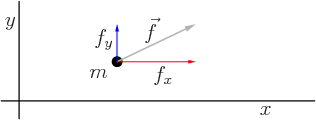
\includegraphics{function_as_vector1}
\caption{Vector $\vec{f}$ as sum of component vectors $\vec{f_x}$ and $\vec{f_y}$.}
\end{figure}

This vector $\vec{f}$ can be expressed as sum of its projection onto axes x and y (respectively $\vec{f_x}$ and $\vec{f_y}$. These two component vectors can be represented in a different way, called \textit{spike diagram}:

\begin{figure}[ht]
\centering
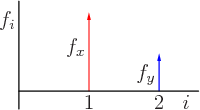
\includegraphics{function_as_vector2}
\caption{Component vectors presented in spike diagram.}
\end{figure}

We can notice, that with each new dimension added to the space, in which the vector is considered, we just add one new spike in the spike diagram representation. Below is given an example of vector in 3D space and another one in space with much larger number of dimensions:

\begin{figure}[ht]
\centering
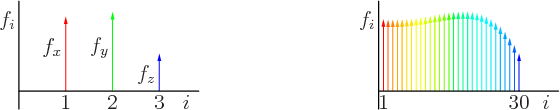
\includegraphics[scale=0.75]{function_as_vector3}
\caption{Left: vector in 3D space. Right: vector in many-dimensional space.}
\end{figure}

If we follow this reasoning, we can consider a vector with an infinite number of dimensions as a spike diagram with infinitely many spikes. This can be in turn represented on a continuous coordinate (e.g. \textit{x}):

\begin{figure}[ht]
\centering
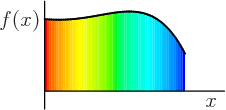
\includegraphics{function_as_vector4}
\caption{Vector with infinite number of dimensions.}
\end{figure}

We can see, that top boundary of the area made of spikes is some function $f(x)$. We have received a direct transition between the concept of a vector and a function - a function can be seen as a vector with infinitely many dimensions. It is worth noticing, that each function can be understood as a vector, but not the other way.

In this work, even when discussing functions, we will represent them in the form of vectors. We will give examples in 2D and 3D spaces, whose aim is to develop intuition about the discussed concept and which can be expanded to a larger number of dimensions.

\subsection{Complex and Hermitian conjugates}

\begin{example}
For a given vector $z$ in a complex space we can create a \textbf{complex conjugate} of such a vector (noted as $\overline{z}$ or $z^*$) in the following way:

\begin{figure}[ht]
\centering
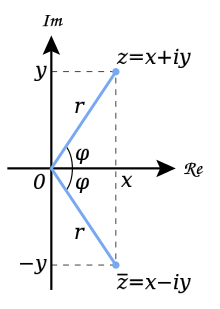
\includegraphics[scale=0.5]{complex_conjugate}
\caption{A vector \textit{z} and its complex conjugate.}
\end{figure}

We can write this in a matrix form as:

\[ z_1 = \begin{pmatrix} 10 \\ i \end{pmatrix}, \ z_{1}^* = \begin{pmatrix} 10 \\ -i \end{pmatrix}  \]

\[ z_2 = \begin{pmatrix} e^{i} \\ i \end{pmatrix}, \ z_{2}^* = \begin{pmatrix} e^{-i} \\ -i \end{pmatrix}  \]
\end{example}

\begin{example}
In a similar way, for a vector \textit{z} we can introduce its \textbf{Hermitian conjugate} as

\[ z = \begin{pmatrix} e^{i} \\ i \end{pmatrix}, \ z^{\dagger} = \begin{pmatrix} e^{-i} & -i \end{pmatrix}, \]

which is equivalent to apply a complex conjugate and a transposition
\[  z^\dagger = (z^*)^T. \]
\end{example}

\begin{example}
The same procedure can be applied to matrices:
\[ M = \begin{pmatrix} 1 & i \\ e^i & 2 \end{pmatrix}, \ M^* = \begin{pmatrix} 1 & -i \\ e^{-i} & 2 \end{pmatrix} \]
\[ M^\dagger = \begin{pmatrix} 1 & e^{-i} \\ -i & 2 \end{pmatrix} \]
\end{example}

\subsection{A vector space and a function space}

\begin{definition}
Let $(\mathbb{F}, +, \cdot)$ be a field (reader can think of this as real or complex numbers). Let X be any nonempty set. Elements of $\mathbb{F}$ and X will be called respectively scalars and vectors. Let's introduce two two-argument operations:
\begin{enumerate}
    \item addition of vectors: $X \times X \rightarrow X$ noted as $x + y$ for $x, y \in X$,
    \item multiplication by scalar: $\mathbb{F} \times X \rightarrow X$, noted as $a \cdot x$ for $a \in \mathbb{F}$ and $x \in X$.
\end{enumerate}
Set X with operations $+$ and $\cdot$ is called a \textbf{vector space} (or \textbf{linear space}) if for any $a,b \in \mathbb{F}$ and $x,y,z \in X$ it fulfills following conditions:
\begin{legal}
    \item $x + y = y + x$ (commutative property),
    \item $x + (y + z) = (x + y) + z$ (associative property of addition),
    \item there exists element $0 \in X$, such that for any $x \in X$, $x + 0 = x$,
    \item for any $x \in X$ exists an opposite element $-x \in X$, such that $x + (-x) = 0$,
    \item $a(x + y) = ax + ay$ (left-distributive property),
    \item $(a + b)x = ax + bx$ (right-distributive property),
    \item $a(bx) = (ab)x$ (associative property of multiplication),
    \item there exists a scalar $1 \in \mathbb{F}$, such that for any $x \in X$, $1 \cdot x = x$.
\end{legal}
Such a vector space is going to be noted as $\langle X, +, \cdot \rangle$.
\end{definition}

\begin{remark}
When we consider fields of real or complex numbers it will be noted respectively $\mathbb{F} = \mathbb{R}$ and $\mathbb{F} = \mathbb{C}$.
\end{remark}

\begin{definition}
Let V be a vector space over the field $\mathbb{F}$ and let X be some set. A set of functions $\{f: X \rightarrow V\}$ with two operations:
\begin{legal}
    \item addition of functions: \\ 
    For any two functions $f, g: X \rightarrow V$, for any $x \in X$, there is a function $h: X \rightarrow V$, such that $h(x) = f(x) + g(x)$,
    \item multiplication of a function by a scalar: \\
    For any function $f: X \rightarrow V$ and scalar $a \in \mathbb{F}$ there is a function $h: X \rightarrow V$ such that $h(x) = a \cdot f(x)$,
\end{legal}
is called a \textbf{function space}.
\end{definition}

\begin{remark}
Function space can be understood as a vector space, whose points are functions.
\end{remark}

It is important to notice, that a term \textit{vector} from the definition of a \textit{vector space} has to be understood differently from the common concept of a vector (arrow with given length, attachment point and direction). In our understanding \textit{vector} is any object, that meets the requirements of vector space, so it can be e.g. a square matrix $n \times n$, a function or a point.

Another noteworthy issue is the \textit{geometric interpretation of vector}. It is very convenient way to visualize a vector as an arrow in e.g. an euclidean 3D space, but this method does not hold for all vector spaces. First of all, it is hard to visualize a vector in more than three dimensions. Secondly, the \textit{direction} property of a vector diminishes, when we are considering unordered fields. Such a field is for example a field of complex numbers $\mathbb{C}$. Let's say, that we can introduce order in the $\mathbb{C}$ field. We have to notice, that $\mathbb{R}$ is a subset of $\mathbb{C}$, so the order imposed on $\mathbb{C}$ should be also correct for $\mathbb{R}$. Unfortunately, this is not possible. Such an order should harmonize with operations of addition and multiplication in these fields. But it is obvious, that for $\mathbb{R}$ we have, that $\forall x \in \mathbb{R}\  x^2 \geq 0$, which does not hold for $\mathbb{C}$ (e.g. $i^2 < 0$). As a result, when we cannot compare two numbers in $\mathbb{C}$ it is incorrect to talk about vector's direction.

\begin{definition}
For a given vector space X over the field $\mathbb{F}$ we define \textbf{basis} as a subset $B \subseteq X$ such that:
\begin{legal}
    \item B is linearly independent,
    \item any $x \in X$ can be written as a linear combination of elements $b \in B$.
\end{legal}
\end{definition}

\subsection{Operators and functionals}

\begin{definition}
Let X and Y be two vector spaces over the field $\mathbb{F}$. A projection $\hat{T}: X \rightarrow Y$ is called a \textbf{linear operator} if for any $x,y \in X$ and $a \in \mathbb{F}$
\begin{legal}
    \item $\hat{T}(x + y) = \hat{T}(x) + \hat{T}(y)$ (additivity),
    \item $\hat{T}(ax) = a\hat{T}(x)$ (homogeneity).
\end{legal}
If $Y = \mathbb{F}$ and T takes the form $\hat{T}: X \rightarrow \mathbb{F}$ it is called a \textbf{functional}.
\end{definition}

\begin{remark}
A functional can be understood as a special case of operator, which instead of returning vector returns scalar (or one-dimensional vector).
\end{remark}

\begin{example}
A simple example of an operator is a \textit{differential operator}, which takes as an input one function and returns the other one:
\[ \frac{d}{dx} f(x) = g(x). \]
\end{example}

\begin{example}
An \textit{integral} is a great example of a functional (it takes some function \textit{f} as an input and returns a number).
\end{example}

From the above definition we know, that an operator takes a vector as its input and outputs some other vector. This operation can be expressed in the form of a matrix.

\begin{example}
Let's say we have an operator $\hat{T}$ and vectors $a = \begin{pmatrix} 1 \\ 2 \end{pmatrix}$ and $b = \begin{pmatrix} 5 \\ 11 \end{pmatrix}$. We have, that
\[ \hat{T}(a) = b, \]
which can be expressed in the matrix form
\[ \hat{T}\begin{pmatrix} 1 \\ 2 \end{pmatrix}  = \begin{pmatrix} 5 \\ 11 \end{pmatrix}.\]
We can see, that $\hat{T}$ can be expressed as a matrix $\begin{pmatrix} 1 & 2 \\ 3 & 4 \end{pmatrix}$:
\[ \begin{pmatrix} 1 & 2 \\ 3 & 4 \end{pmatrix} \begin{pmatrix} 1 \\ 2 \end{pmatrix} = \begin{pmatrix} 5 \\ 11 \end{pmatrix}. \]
\end{example}

Action of an operator can be understood in two ways:
\begin{legal}
    \item it rotates the vector around the basis:
    \begin{figure}[ht]
        \centering
        \begin{minipage}{.5\textwidth}
          \centering
          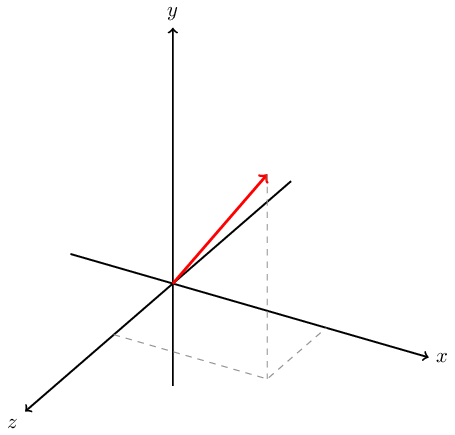
\includegraphics[width=.6\linewidth]{original_vector}
          \captionof{figure}{Original vector.}
        \end{minipage}%
        \begin{minipage}{.5\textwidth}
          \centering
          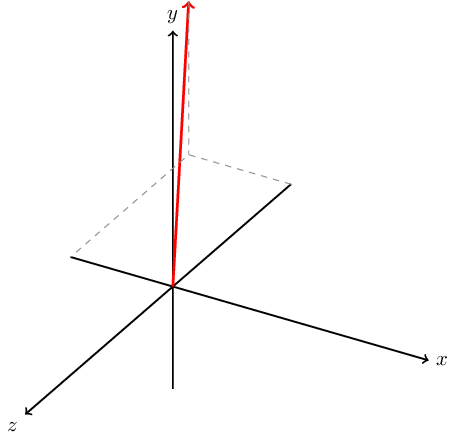
\includegraphics[width=.6\linewidth]{rotated_vector}
          \captionof{figure}{Rotated vector.}
        \end{minipage}
    \end{figure}
    \item it rotates the basis and leaves the vector unchanged:
    \begin{figure}[ht]
        \centering
        \begin{minipage}{.5\textwidth}
          \centering
          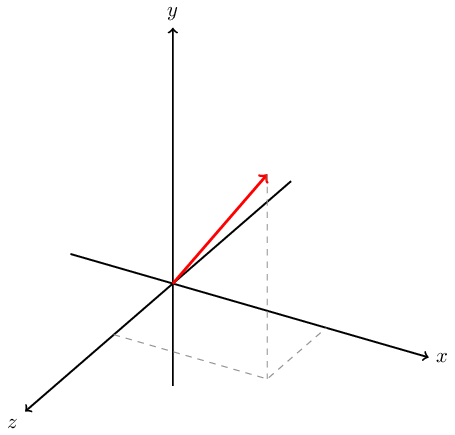
\includegraphics[width=.6\linewidth]{original_vector}
          \captionof{figure}{Original vector.}
        \end{minipage}%
        \begin{minipage}{.5\textwidth}
          \centering
          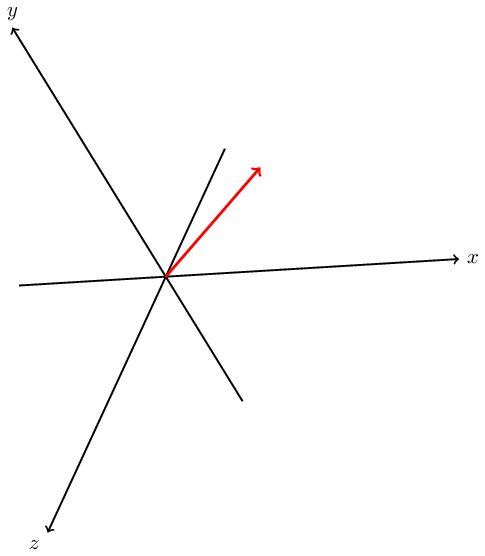
\includegraphics[width=.6\linewidth]{rotated_basis}
          \captionof{figure}{Rotated basis.}
        \end{minipage}
    \end{figure}
\end{legal}

\subsection{From a vector space to a Hilbert space}

In this subsection we will gradually expand definition of a vector space with new features and finally we will introduce an inner product space, which will be essential in next chapters (however the concept of topological space will not be discussed in this work). Relationships between different kinds of spaces are given in the picture below.

\begin{figure}[ht]
\centering
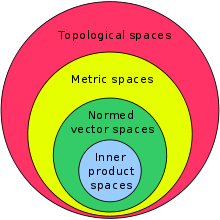
\includegraphics{spaces}
\caption{Relationships between spaces.}
\end{figure}

\begin{definition} \label{metric_space}
Let X be a nonempty set and d be a functional, $d: X \times X \rightarrow \mathbb{F}_{0}$ (where $\mathbb{F}_0$ are non-negative elements of field $\mathbb{F}$), called a \textbf{metric} (or a distance), if it meets the following requirements (for any $x,y,z \in X$):
\begin{legal}
    \item $d(x, y) = 0$ if and only if $x = y$,
    \item $d(x, y) = d(y, x)$,
    \item $d(x, y) \leq d(x, z) + d(z, y)$.
\end{legal}

A set X with a metric d is called a \textbf{metric space} and is noted as $\langle X, d \rangle $.
\end{definition}

\begin{definition}
For a set X let us consider sequence $(x_i)$, where $x_i \in X$. Such sequence is called \textbf{Cauchy sequence}, if
\[ \forall_{\epsilon > 0} \ \exists_{N \in \mathbb{N}} \ \forall_{m,n > N} \ d(x_m, x_n) < \epsilon. \]
\end{definition}

\begin{definition}
A metric space $\langle X, d \rangle$ is called \textbf{complete}, if every Cauchy sequence converges to an element of X.
\end{definition}

\begin{definition}
Let X be a vector space over the field $\mathbb{F}$. We define a functional performing $ x \rightarrow \norm{x}$, where $ x \in X$ and $\norm{x}$ is a non-negative element of X. It is called a \textbf{norm}, if for any $x,y \in X$ and $a \in \mathbb{F}$ it has the following properties:
\begin{legal}
	\item $\norm{x}$ = 0 implies $x = 0$,
	\item $ \norm{x + y} \leq \norm{x} + \norm{y}$ (triangle inequality),
	\item $\norm{ax} = |a| \cdot \norm{x}$ (norm is homogeneous).
\end{legal}
\end{definition}

\begin{definition}
A pair $\langle X, \norm{\cdot} \rangle$, where X is a vector space and $\norm{}$ is a norm in it, is called a \textbf{normed space}.
\end{definition}

\begin{definition}
Let X be a vector space over the field $\mathbb{F}$ with a functional $f: X \times X \rightarrow \mathbb{F}$ noted as $\langle x | y \rangle$ for $x,y \in X$. If f meets the following requirements:
\begin{legal}
    \item $\langle x + y | z\rangle = \langle x | z \rangle + \langle y | z \rangle$,
    \item $\langle ax | y \rangle = a\langle x | y \rangle$,
    \item $\langle y | x\rangle = \langle x | y \rangle^\dagger$,
    \item $\langle x | x \rangle > 0$ for $x \neq 0$,
\end{legal}
it is called an \textbf{inner product} (or a \textbf{dot product}) and the pair $\langle X, \langle\cdot | \cdot\rangle \rangle$ is called an \textbf{inner product space}. When $\langle X, \langle\cdot | \cdot\rangle \rangle$ is over the field $\mathbb{C}$, the name \textbf{unitary space} is used, when referring to it.
\end{definition}

\begin{remark}
An inner product can be understood in terms of vectors projection. Below is given an example in Euclidean space:


\begin{figure}[ht]
\centering
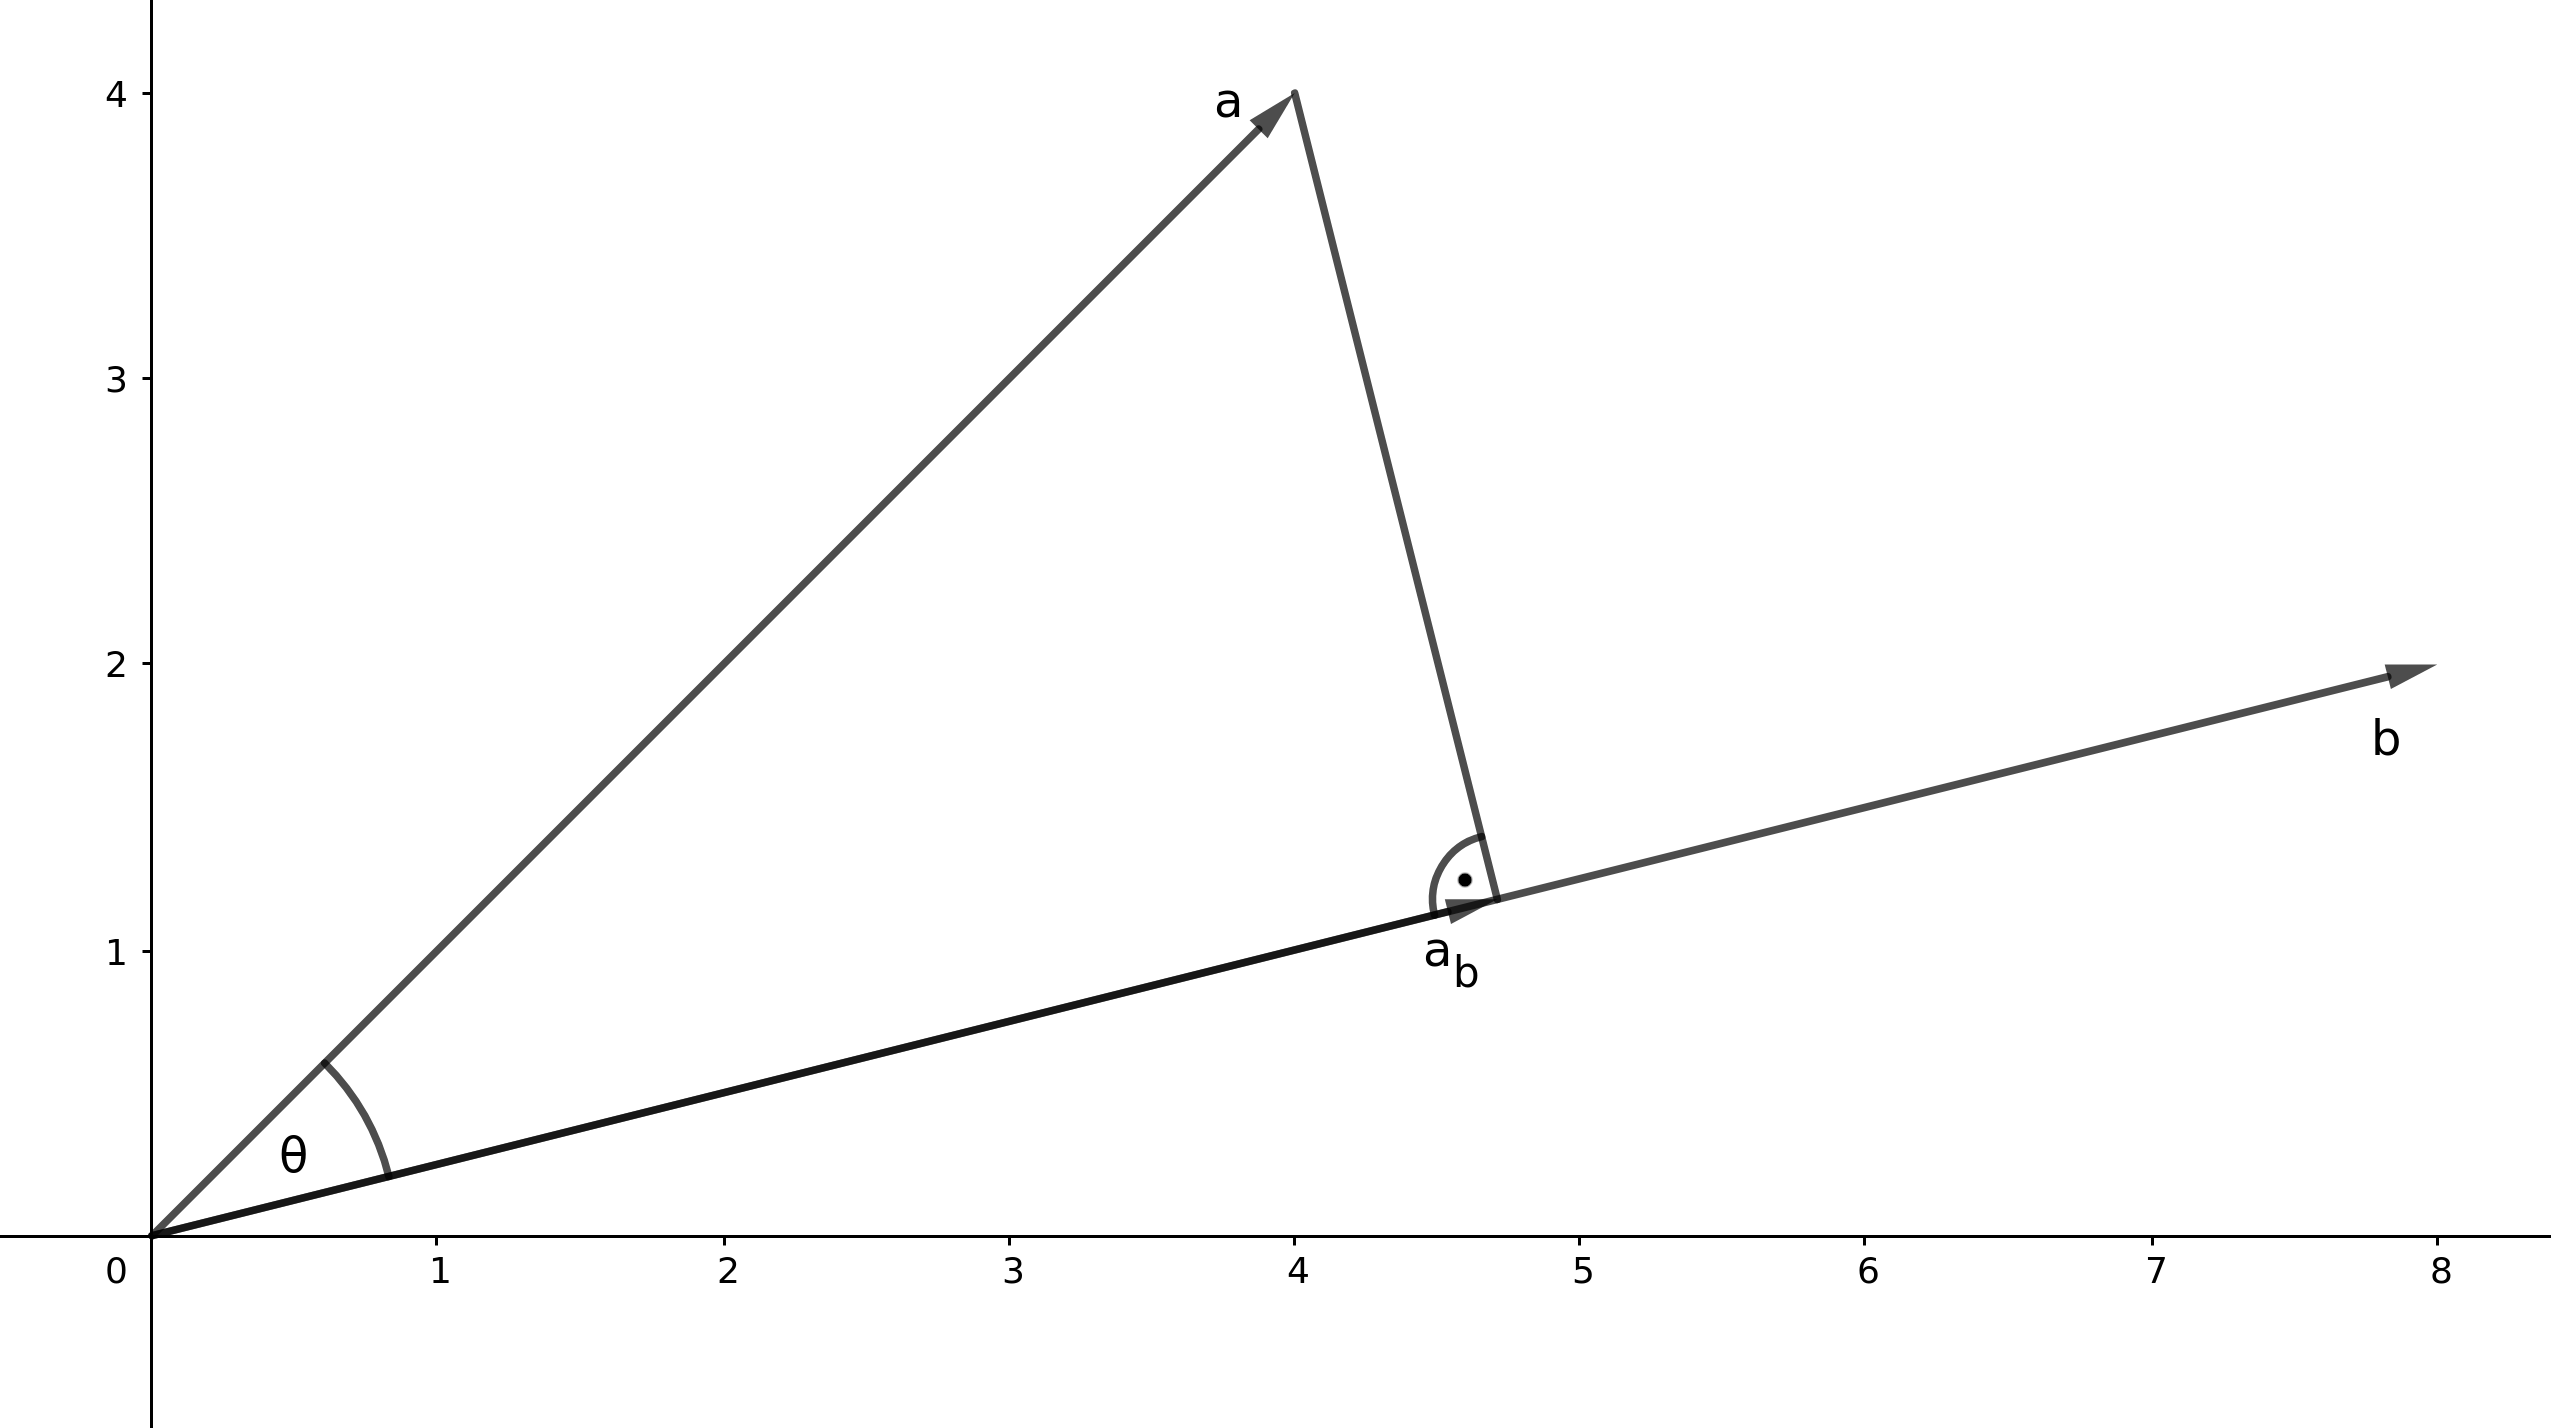
\includegraphics[scale=0.15]{vectors_projection}
\caption{A geometrical interpretation of inner product.}
\end{figure}

In such a case, we define an inner product as
\[ \boxed{\langle a | b\rangle = \norm{a} \norm{b} cos(\theta)}.\]

We can see, that 
\[\norm{a_b} = cos(\theta) \norm{a}, \] 
so 
\[ \boxed{\langle a | b\rangle = \norm{a} \norm{b} cos(\theta) = \norm{a_b} \norm{b}}. \]

We have shown, that an inner product can be understood as a multiplication of the norm of projection of the vector a onto b and the norm of the vector b.

Let's consider an inner product $\langle a | a \rangle$. As shown above, it can be understood as a projection of the vector a onto itself. Due to this, a result of such an operation equals

\[ \langle a | a \rangle = \norm{a_a} \norm{a} = \norm{a} \norm{a} = \norm{a}^2.  \]

This implies, that a norm in an inner product space is defined as

\[ \boxed{\norm{a} = \sqrt{\langle a | a \rangle}}.  \]
\end{remark}

\begin{definition}
If an inner product space X is complete due to the metric induced by the inner product (through the norm) it is called a \textbf{Hilbert space}.
\end{definition}

\begin{remark}
We have previously shown the dependence between a norm and an inner product
\[ \norm{x} = \sqrt{\langle x | x \rangle}. \]
It is important to notice, that a \textbf{norm is a real-valued functional}. When we say, that a metric is induced by a norm, it can be written as
\[  d(x, y) = \norm{x - y} = \sqrt{\langle x-y | x-y \rangle}. \]
\end{remark}

\begin{remark}
An inner product in a Hilbert space is defined as follows
\[ \langle x | y \rangle = x^\dagger y.\]
An inner product defined in such a way always returns real-valued numbers (even when a Hilbert space is over the field $\mathbb{C}$).
\end{remark}

\subsection{Normalization, ortogonality and orthonormality of vectors}

\begin{definition}
Let $\langle X, \langle \cdot | \cdot \rangle \rangle$ be an inner product space over the field $\mathbb{F}$ and $x,y \in X$. We say, that x and y are \textbf{orthogonal}, if $\langle x | y\rangle = 0$. We denote this as $x \perp y$.
\end{definition}

\begin{definition}
Let $\langle X , \norm{\cdot} \rangle$ be a normed space. An \textbf{unitary vector} v (also called a \textbf{versor}) is a vector, for which $\norm{v} = 1$.
\end{definition}

\begin{remark}
For any vector v (from a normed space) we can define a procedure called a \textbf{normalization}, thanks to which it can be changed to unitary vector $v^0$:
\[ v^0 = \frac{v}{\norm{v}} = \frac{v}{\sqrt{\langle v | v \rangle}} \]
\end{remark}

\begin{remark}
When all of the vectors $\{v_i\}_{i=1}^n$ spanning a vector space (base vectors) have a length equal to 1 ($\norm{v_i} = 1$), we call such a base a \textbf{normalized base}.
\end{remark}

\begin{definition}
Let $\langle X, \norm{\cdot} \rangle$ be a normed space and $x,y \in X$. We say, that x and y are \textbf{orthonormal}, when
\[ \langle x | y \rangle = 
\begin{cases} 
    1, & if \  x = y \\
    0, & if \  x \neq y
\end{cases}
\]
An orthonormality is just an extension of an ortogonality (two vectors are ortogonal and have a length equal to 1).
\end{definition}

\begin{remark}
A normalized base is a base made of orthonormal vectors.
\end{remark}

\subsection{Unitary and Hermitian operators}

\begin{definition}
We say, that for vector spaces X and Y, an operator $\hat{T}: X \rightarrow Y$ is \textbf{unitary}, if the following occurs
\[ \hat{T}\hat{T}^\dagger = I, \]
where I is the identity operator. I may be understood as the identity matrix
\[ I = \begin{pmatrix} 1 & 0 \\ 0 & 1 \end{pmatrix}.  \]
\end{definition}

\begin{remark} \label{unitary_operators_no_length_change}
This remark is extremely important because of the correct understanding of the further part of the work. \textbf{Unitary operators applied to vectors do not change their length} (vectors are only \textbf{rotated}).
\end{remark}

\begin{definition}
For vector spaces X and Y, an operator $\hat{T}: X \rightarrow Y$ is called \textbf{Hermitian} (or \textbf{self-adjoint}), if
\[ \hat{T} = \hat{T}^\dagger. \]
\end{definition}

\subsection{Eigenvector, eigenfunction and eigenvalue of an operator}

\begin{definition}
For any operator $\hat{T}$ we can write the following linear equation:
\[ \hat{T} x = \lambda x, \]
where x is called an \textbf{eigenvector} and $\lambda$ is called an \textbf{eigenvalue}.
When we are considering a function space instead of a vector space, the above equation takes the following form:
\[  \hat{T} f = \lambda f, \]
and f is called an \textbf{eigenfunction}.
\end{definition}

\newpage
\section{Basics of quantum mechanics}

We will begin this section by introducing some notation. Later, we will present six postulates of quantum mechanics, after which we will provide an example illustrating a counter-intuitive behavior of quantum entities. Finally, we will explain the use of a tensor product in the description of more complicated physical systems and give a short introduction to the concept of entaglement.

\subsection{Bra-ket notation, Kronecker and Dirac deltas}

\begin{definition}
Every vector $\vec{x}$ can be written in the form
\[ | x \rangle \equiv \begin{pmatrix} x_1 \\ x_2 \\ \cdot \\ \cdot \\ \cdot \\ x_n \end{pmatrix}, \]
which is called the \textbf{ket} notation.
\end{definition}

\begin{definition}
Any Hermitian conjugate of a vector $\vec{x}$ can be written as
\[ \langle x | \equiv \begin{pmatrix} x_1^* & x_2^* & \cdot \cdot \cdot & x_n^* \end{pmatrix}, \]
which is called the \textbf{bra} notation.
\end{definition}

\begin{remark}
We have previously stated, that an inner product in Hilbert spaces is defined as
\[ \langle x | y \rangle = x^\dagger y.\]
Note, that it can be also written in the bra-ket notation in the following way
\[ \langle x | y \rangle = \begin{pmatrix} x_1^* & x_2^* & \cdot \cdot \cdot & x_n^* \end{pmatrix} \begin{pmatrix} y_1 \\ y_2 \\ \cdot \\ \cdot \\ \cdot \\ y_n \end{pmatrix} = x^\dagger y,\]
which is consistent with the notation, which we used earlier to denote the inner product.
\end{remark}


\begin{definition}
We define a symbol called \textbf{Kronecker delta} (noted as $\delta_{ij}$) in the following way
\[ \delta_{ij} = \begin{cases}
    0,\ if\ i \neq j \\
    1,\ if\ i = j
\end{cases} \]
\end{definition}

\begin{definition}
We define a \textbf{Dirac delta function} as
\[ \delta(x) = \begin{cases}
    +\infty, \ if \ x = 0 \\
    0, \ \ \ \ \ if \ x \neq 0
\end{cases}\]
with an additional constraint
\[ \int_{-\infty}^{+\infty} \delta(x)dx = 1. \]
\end{definition}

\subsection{Postulates of quantum mechanics}

When describing a mathematical model simulating quantum physics we use Hilbert spaces over the field $\mathbb{C}$ (that is why we needed to introduce all the definitions in the previous section). At the beginning it is important to notice, that although we are operating in a space with complex numbers, a result of an inner product is always real-valued. This property of the Hilbert space is indispensable, while creating model with a practical application, because results of measurements of physical systems are always real-valued.

Below we introduce six postulates, which for quantum physics are what axioms for mathematics are.

\begin{postulate}
State of a physical system can be represented by a \textbf{state function} $|\psi \rangle$, also called a \textbf{wave function}. It has to be continuous and differentiable. It contains all possible information about the system.
\end{postulate}

\begin{definition}
Every measurable physical property T is called an \textbf{observable}. It can be understood as e.g. an energy, a momentum, a mass or an angular momentum.
\end{definition}

\begin{postulate}
Every observable T is described by an operator $\hat{T}$. 
\end{postulate}

\begin{postulate}
Every measurement of an observable T can only give one of the eigenvalues $\lambda$ of the operator $\hat{T}$ (associated with this physical property), that is
\[ \hat{T} |\psi\rangle = \lambda |\psi \rangle,  \]
where $|\psi \rangle$ is an eigenfunction of the operator $\hat{T}$.
\end{postulate}

\begin{postulate}
The probability, that measurement will return an eigenvalue $\lambda$ is equal to $| \langle \psi_\lambda | \psi \rangle |^2$, where $\langle \psi_\lambda | \psi \rangle = c_\lambda$ is called a \textbf{probability amplitude}.
\end{postulate}

\begin{remark}
We say, that a system before measurement is in a \textbf{superposition} of all eigenfunctions (that is, it is a sum of all its eignefunctions). It can be written, as
\[ | \psi \rangle = \sum_n \langle \psi_n | \psi \rangle |\psi_n \rangle = \sum_n c_n | \psi_n \rangle. \]
Usually eigenstates are normalized, so
\[ \langle \psi_i | \psi_j \rangle = \delta_{ij}. \]
When we are considering a case with a continuous set of egienstates, we have to use the Dirac's $\delta$-function
\[ \langle \psi_i | \psi_j \rangle = \delta(\psi_i - \psi_j). \]
If eigenfunctions are normalized, we can write (for a discrete case of measurements' results)
\[ \sum_n c_n = 1. \]
While considering a probability of finding a result of a measurement of an observable T in an interval [T, T + dT] equal to P(T)dT, we obtain
\[ \int_{-\infty}^{+\infty} P(T)dT = 1. \]
A set of normalized eigenfunctions is said to create a basis of the wave function $| \psi \rangle$.
\end{remark}

\begin{definition}
We designate the \textbf{expected value} of an observable T as $\langle T \rangle$. If measurements of T return discrete values $T_i$ (with the same probability), it can be written as
\[  \langle \hat{T} \rangle = \frac{1}{N} \sum_{i = 1}^N T_i,\]
where N is a number of all possible outcomes. It can be also expressed in terms of probability $P(T_i)$
\[ \langle \hat{T} \rangle = \sum_{i=1}^N T_i P(T_i). \]
If results of a measurement of T create a continuous set, we denote this as
\[ \langle \hat{T} \rangle = \int_{-\infty}^{+\infty} T P(T) dT, \]
where P(T) is a probability density function. Concluding from the above we can say, that P(T)dT is a probability of obtaining T in the interval [T, T + dT]. 
\end{definition}

\begin{remark}
We write the expected value of an observable T (for a discrete case) as
\[ \langle \hat{T} \rangle = \langle \psi | \hat{T} | \psi \rangle = \sum_{i} \sum_{j} c_i^*c_j \langle \psi_i | \hat{T}|\psi_j\rangle = \sum_{i} \sum_{j} c_i^* c_j \langle \psi_i | \psi_j \rangle \lambda_j = \sum_{i} |c_i|^2 \lambda_i \]
Now, we are going to use the equation for calculating the eigenfunction of $\hat{T}$
\[ \hat{T} |\psi_n \rangle = \lambda_n |\psi_n \rangle, \]
where $|\psi_n \rangle$ is the n-th eigenfunction of the operator $\hat{T}$. We obtain
\[ \sum_n \psi_n^* \hat{T} \psi_n = \sum_n \psi_n^* \lambda_n \psi_n = \sum_n \lambda_n \psi_n^* \psi_n = 
\sum_n \lambda_n | \langle \psi_n | \psi_n\rangle |^2 = \sum_n \lambda_n | c_n |^2 .\]
Summarizing we can write, that in a discrete case, the expected value of an observable T equals to
\[ \boxed{\langle \hat{T} \rangle = \sum_n \lambda_n | c_n |^2} \]
This reasoning can be extended to the case with a continuous set of measurements' results
\[ \langle \hat{T} \rangle = \int_{-\infty}^{+\infty} T P(T) dT. \]
\end{remark}

\begin{postulate}
A measurement of an observable of a physical system (associated with an operator $\hat{T}$), returning a value $\lambda$, leaves this system in a state $|\psi_\lambda \rangle$, where
\[ \hat{T} |\psi_\lambda\rangle = \lambda \ |\psi_\lambda\rangle \]
($|\psi_\lambda \rangle$ is the eigenfunction of the operator $\hat{T}$, corresponding to the eigenvalue $\lambda$). This is often referred as to a \textbf{collapse} of the system.
\end{postulate}

\begin{postulate}
A wave function of a physical system depends on a time according to the \textbf{time dependent Schr\"odinger equation}
\[ i\hbar \frac{\partial}{\partial t}\psi(\vec{r}, t) = \hat{H}\psi(\vec{r}, t), \]
where $\psi(r, t)$ is a wave function dependent from a position $\vec{r}$ and a time t and $\hat{H}$ is an energy operator called \textbf{hamiltonian}.
\end{postulate}

\newpage
\subsection{Illustrative example - Stern-Gerlach experiment}

This experiment measures the magnetic moment caused by the spin of an elementary particle, called \textbf{spin magnetic moment}. To better understand this property, reader can visualize it as a spinning electron (although this analogy is not completely correct). Particles can only have quantized (discrete) values of a spin. Electrons are said to have a spin $+\frac{1}{2}$ or $-\frac{1}{2}$, which is denoted as $| + \rangle$ and $|-\rangle$ respectively. Because of this, a state of an electron's spin before a measurement can be written as
\[ | \psi \rangle = \frac{1}{\sqrt{2}}(|+\rangle + |-\rangle ), \]
which is equal to
\[ |\psi \rangle = \begin{pmatrix} \frac{1}{\sqrt{2}} \\  \frac{1}{\sqrt{2}} \end{pmatrix}. \]
Values next to the possible outcomes $|+\rangle$ and $|-\rangle$ are equal to $\frac{1}{\sqrt{2}}$, because a measurement returns each of these options with probability $|\frac{1}{\sqrt{2}}|^2$, so an electron have a 50\% probability of having a spin $|+\rangle$ and 50\% of having a spin $|-\rangle$.
\begin{remark}
As mentioned in the previous subsection, an electron before a measurement is in a \textbf{superposition} of states having spins $|+\rangle$ and $|-\rangle$. During the experiment it collapses to only one of the possible outcomes.
\end{remark}

When an electron moves in a presence of a magnetic field, because of its spin it will deflect in some direction. We can introduce a device, which uses this phenomenon to measure an electron's spin along a given axis. We can create such a field, that an electron in its presence will deflect upwards, if it has a $|+\rangle$ spin along z axis, and downwards, if it has a $|-\rangle$ spin. It will be presented as a black-box

\begin{figure}[ht]
\centering
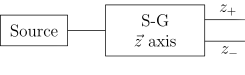
\includegraphics{stern_gerlach_device}
\caption{A Stern-Gerlach device recognizing the electron's spin along z axis.}
\end{figure}

A notation $z_+$ means, that an electron has the spin $|+\rangle$ along z axis and $z_-$, that it has the $|-\rangle$ spin along z axis. For the purpose of this thought experiment Let's assume, that an electron is in a state $|\psi \rangle$ mentioned above ($| \psi \rangle = \frac{1}{\sqrt{2}}(|+\rangle + |-\rangle )$). In such a case, an electron has 50\% chances of deflecting upwards, and 50\% of deflecting downwards. \newline

When an electron's spin collapses after the experiment in one of the possible outcomes, next experiments (measuring the same property) will return the same result

\begin{figure}[ht]
\centering
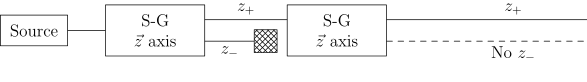
\includegraphics[scale=0.7]{stern_gerlach_consecutive_z_axis.png}
\caption{Two consecutive measurements of the electron's spin along z axis.}
\end{figure}

In the above experiment, after the first measurement the electron's spin collapsed to the state $|+\rangle$ (along z axis) and because of this, the second measurement of this property returned the same result.\newline

Another important phenomenon, is that a measurement of a spin along one axis does not affect the result of a measurement along other axes.

\begin{figure}[ht]
\centering
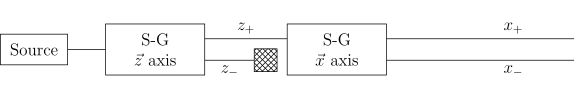
\includegraphics[scale=0.7]{stern_gerlach_different_axes}
\caption{Two consecutive measurements of the electron's spin along different axes.}
\end{figure}

In the experiment above the electron had the $|+\rangle$ spin along z axis, but it did not influence the measurement of the spin along x axis (it still had 50\% chances of having the $|+\rangle$ spin and 50\% of having the $|-\rangle$ spin).\newline

Finally, a measurement of a spin along one axis erases all information gathered about this property along other axes. It is presented at the picture below

\begin{figure}[ht]
\centering
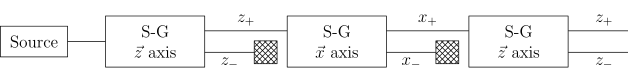
\includegraphics[scale=0.7]{stern_gerlach_deletion_of_information}
\caption{The deletion of information about the electron's spin along z axis.}
\end{figure}

In the first measurement the electron had the $|+\rangle$ spin along z axis. Later, the spin along x axis was measured, which made, that the electron again had 50\% chances of having the $|+\rangle$ spin and 50\% of having the $|-\rangle$ spin along z axis.

\subsection{Description of compound systems - tensor product and entanglement}

Let's say, we want do describe the behavior of a physical system made up of many simpler systems e.g. an interaction between two elementary particles. We will call all of the possible states, in which the first particle can be, as a set \textit{A}, and all possible states of the second particle as a set \textit{B}. If states of these two quantum entities are independent from each other, the whole system (two particles) can be described as a \textbf{tensor product} of the set A with the set B. On the other hand, if states of these two particles are not independent, we say that they are \textbf{entangled}.

\begin{definition}
The \textbf{tensor product} (or the \textbf{Kronecker's product}) of two matrices A and B, where $A \in M_{m\times n}$ and $B \in M_{k \times l}$ is a block matrix $C \in M_{mk \times nl}$ of the form
\[ C = A \otimes B  = \begin{pmatrix} a_{11} & a_{12} & \cdots & a_{1n} \\
a_{21} & a_{22} & \cdots & a_{2n} \\ \vdots & \vdots & \ddots & \vdots \\ a_{m1} & a_{m2} & \cdots & a_{mn}\end{pmatrix} \otimes \begin{pmatrix} b_{11} & b_{12} & \cdots & b_{1l} \\
b_{21} & b_{22} & \cdots & b_{2l} \\ \vdots & \vdots & \ddots & \vdots \\ b_{k1} & b_{k2} & \cdots & b_{kl}\end{pmatrix} = \]


\[\begin{pmatrix}
a_{11}b_{11} & a_{11}b_{12} & \cdots & a_{12}b_{11} & a_{12}b_{12} & \cdots \\
a_{11}b_{21} & a_{11}b_{22} &  & a_{12}b_{21} & a_{12}b_{22} &  \\
\vdots \\
a_{11}b_{k1} & a_{11}b_{k2} & \cdots & a_{12}b_{k1} & a_{12}b_{k2} \\
\vdots & & & & & \ddots \\
& & & & & & a_{mn}b_{11} & a_{mn}b_{12} & \cdots \\
& & & & & & a_{mn}b_{21} & a_{mn}b_{22} & \cdots \\
& & & & & & \vdots
\end{pmatrix}
\]

\end{definition}

\begin{example}
Let's consider two matrices - $H = \frac{1}{\sqrt{2}}\begin{pmatrix} 1 & 1 \\ 1 & -1 \end{pmatrix}$ and the identity matrix $I = \begin{pmatrix} 1 & 0 \\ 0 & 1 \end{pmatrix}$. Tensor product of these two matrices is equal to 
\[ H \otimes I = \frac{1}{\sqrt{2}}\begin{pmatrix} 1 & 1 \\ 1 & -1 \end{pmatrix} \otimes \begin{pmatrix} 1 & 0 \\ 0 & 1 \end{pmatrix} = \frac{1}{\sqrt{2}} \begin{pmatrix} 1 \cdot 1 & 1 \cdot 0 & 1 \cdot 1 & 1 \cdot 0 \\
1 \cdot 0 & 1 \cdot 1 & 1 \cdot 0 & 1 \cdot 1 \\ 1 \cdot 1 & 1 \cdot 0 & -1 \cdot 1 & -1 \cdot 0 \\ 1 \cdot 0 & 1 \cdot 1 & -1 \cdot 0 & -1 \cdot 1 \end{pmatrix} = \frac{1}{\sqrt{2}}\begin{pmatrix} 1 & 0 & 1 & 0 \\ 0 & 1 & 0 & 1 \\ 1 & 0 & -1 & 0 \\ 0 & 1 & 0 & -1 \end{pmatrix}\]
\end{example}

\begin{example}\label{example_0_1_states}
Let's call vectors $\begin{pmatrix} 1 \\ 0 \end{pmatrix}$ and $\begin{pmatrix} 0 \\ 1 \end{pmatrix}$ as $|0\rangle$ and $|1\rangle$ respectively. Tensor product of these two vectors is equal to
\[ |0\rangle \otimes |1\rangle = \begin{pmatrix} 1 \\ 0 \end{pmatrix} \otimes \begin{pmatrix} 0 \\ 1 \end{pmatrix} = \begin{pmatrix} 1 \cdot 0 \\ 1 \cdot 1 \\ 0 \cdot 0 \\ 0 \cdot 1 \end{pmatrix} = \begin{pmatrix} 0 \\ 1 \\ 0 \\ 0 \end{pmatrix}\]
\end{example}

The above example describes the behavior of two independent particles - first in the state $|0\rangle$ and second in the state $|1\rangle$, considered as one, bigger system. However, it is not always possible to use the tensor product to write a vector characterizing such compound structure. As mentioned before, such a system is called entangled. We can visualize two entangled particles being in a superposition of having a $|+\rangle$ and  a $|-\rangle$ spin along some axis. A measurement of a spin of only one of these particles collapses the whole system. Moreover, it does so in an anti-symmetrical way - when one particle has a $|+\rangle$ spin, the other one has a $|-\rangle$ spin.

The topic of entanglement will be expanded in the second chapter of this work.

\begin{remark}
Sometimes we will denote the tensor product of two states in the following way

\[ |\psi \rangle \otimes |\phi \rangle \equiv |\psi , \phi \rangle. \]
\end{remark}


\newpage
\section{Classical and quantum computational complexity theory}

Computational complexity theory is a branch of the theoretical computer science, that classifies computational problems in classes, depending on the amount of resources that are necessary to solve them. There are two main kinds of resources needed in the computation process - time and memory. An algorithm solving some problem is considered as fast, if it does not exceed the \textit{polynomial} amount of resources (relative to the size of the input data), and the considered problem is thought of as \textit{easy}. On the other hand, problems which need \textit{exponential} amount of resources, are called \textit{hard} problems. 

It is important to notice, that when we are referring to the word "exponential" we allow ourselves for a little misuse of this word. When we name some function in this way, we just mean a function greater than the polynomial one. So, despite the fact that, for example, the function $n^{logn}$ is not exponential (strictly speaking), we will call it in this way when classifying problems.

Reader can argue, why we are naming algorithms using a polynomial amount of resources during the execution, as fast. In fact, adoption of such an approach enables us to create a consistent and elegant way of classifying problems, which would not be possible, if we would choose some other criteria.

We will now present basic computational complexity classes and later, we will try to use them while describing possibilities and limitations of quantum computers.

\begin{definition}
We define the class \textbf{P} (or \textbf{polynomial time}), as a set of problems, that can be solved by a sequential machine in a polynomial time.
\end{definition}

\begin{definition}
Let's say, we have an oracle, that gives solution to a given problem (it does not have to be a correct solution). We say, that a problem is in the \textbf{NP} class (or \textbf{non-deterministic polynomial time}), if there exists a sequential machine, that can verify in a polynomial time, if the solution given by the oracle is correct.
\end{definition}

\begin{definition}
As the \textbf{PSPACE} class, we understand a set of problems, for which exists a sequential machine, returning solution using polynomial amount of memory (but it does not have to run in a polynomial time).
\end{definition}

\begin{definition}\label{BPP}
The \textbf{BPP} class (or \textbf{bounded-error probabilistic polynomial time}) is a set of problems, for which exists a sequential machine, running in a polynomial time, and returning a correct solution with probability greater than or equal to $\frac{2}{3}$.
\end{definition}

\begin{remark}
Let's say, we have a sequential machine for a given problem from the BPP class. As given in the definition above, this machine will return a correct answer to this problem with a probability greater than or equal to $\frac{2}{3}$ and can be wrong with a probability less than or equal to $\frac{1}{3}$. We can notice, that if we run this machine \textit{k} times and compare obtained results, the probability of receiving correct answer is greater than or equal to $(1 - \frac{1}{3})^k$. If we could run these machines in parallel, we would receive a sequential machine running in the same time, as the original one, but returning correct answer to given problem with a probability greater than or equal to $(1 - \frac{1}{3})^k$.
\end{remark}

\begin{definition}
We define the \textbf{quantum circuit} as a computational model, which uses unitary operators on quantum states. It is a quantum mechanical equivalent of a classical circuit made of logical gates, operating on \textit{n} bits.
\end{definition}

\begin{remark}
At this point, reader can think of a quantum circuit as a sequential machine from the previous definitions, which additionally uses the phenomena occurring in quantum physics. This topic will be described in detail in the next chapter.
\end{remark}

\begin{definition}\label{BQP}
The \textbf{BQP} class (or \textbf{bounded-error quantum polynomial time}) is a set of problems, for which exists a quantum circuit, running in a polynomial time, and returning correct solution with a probability greater than or equal to $\frac{2}{3}$.
\end{definition}

\begin{remark}
BQP is a quantum mechanical equivalent of the classical BPP class. Let's say, we have a possibility of preparing a quantum state, being in a superposition of runs of \textit{k} machines from BPP class (before measurement, it is every possible run out of the \textit{k} possible runs). We can modify this state by acting on it with unitary operators (it is like acting on all of the original machines at the same time). Finally, during the measurement we are obtaining a solution, which has a large probability of being correct.
\end{remark}

\begin{remark}
So far it is known, that P is a subclass of BPP, and that BPP is a subclass of PSPACE. However, it wasn't proved, whether these classes are equal or not, which can be written as
\[ P \subseteq BPP \subseteq PSPACE. \]
Additionally it was shown, that quantum computers can solve problems from P efficiently, but cannot solve problems outside PSPACE in a fast way \cite{nielsen_chuang}. While comparing the definition \ref{BPP} with the definition \ref{BQP} it is obvious, that BPP is a subclass of BQP (but it is not known, if they are equal). Above statements led us to write following relations
\[ BPP \subseteq BQP \subseteq PSPACE.\]
If we could prove, that $BPP \neq BQP$ we would automatically obtain, that $BPP \neq PSPACE$. It would be an outstanding result, because the analysis of how quantum computational complexity classes fit in the classical model of computation would provide us with answers about the relationships between the classical classes!
\end{remark}

The suspected relationship between the BQP and classical computational complexity classes is given at the picture below.

\begin{figure}[ht]
\centering
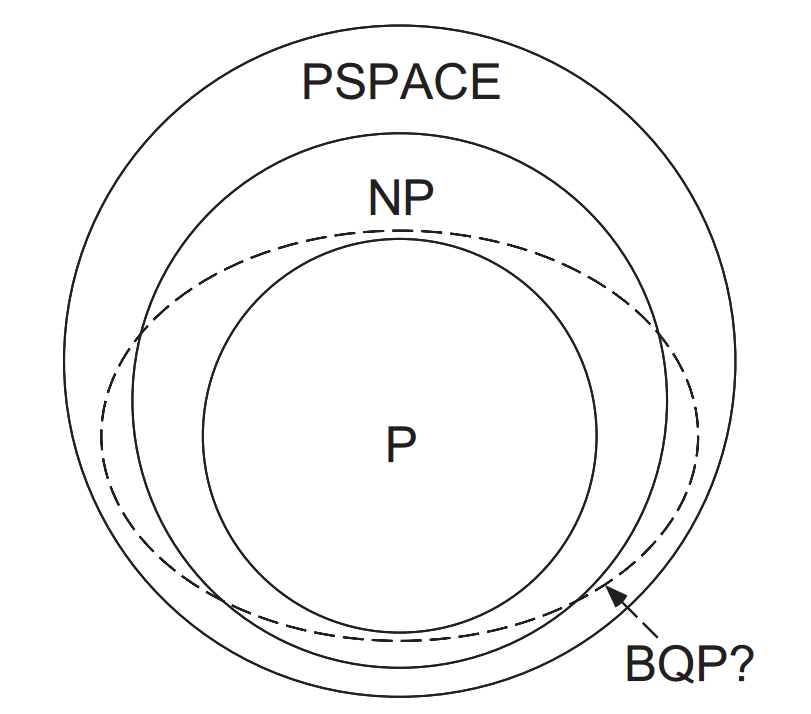
\includegraphics[scale=0.4]{classical_and_quantum_classes_relations}
\caption{The suspected relationship between the BQP and classical computational complexity classes.}
\end{figure}

\begin{definition}
Let's say, we are given an oracle returning a solution to a given problem (as previously, it does not have to be a correct solution). The \textbf{QMA} class (for \textbf{quantum Merlin Arthur}) is a set of problems, for which a solution given by the oracle can be verified by a quantum circuit in a polynomial time. The circuit has a probability of being correct greater than $\frac{2}{3}$.
\end{definition}

\begin{remark}
Although the BQP class is closer to the classical BPP class, we can see that relation between BQP and QMA is similar to the relation between P and NP. Because of this, these two classes are sometimes called as quantum equivalents of P and NP (BQP and QMA respectively).
\end{remark}


Final property of quantum computers, which will be discussed in this work, is their ability to speed up the process of finding solutions for problems from NP. The idea is, that we can generate each possible solution to a given problem, and then check each of them, whether it is correct or not (it is referred to as \textbf{brute force} method). Although, the amount of possible solutions for problems from NP is exponential, we will show in section \ref{quantum_search_algorithm}, that quantum computing provides a quadratic speed up in such a process.


